% =====================================================================
% FAIR 2026 — 7-minute oral presentation
% Paper: papers/fair2026/manuscript/main_en.tex
% Compile: ./compile.sh   (XeLaTeX; notes version via NOTES=1 ./compile.sh)
%
% TIMING PLAN (7:00 total, ~30 s buffer). Three section pages sit between
% the parts; they are not frame-numbered and cost ~5 s each to click past.
%   Title .......................... 0:20
%   I   Problem, contributions ..... 1:25   (2 slides)
%   II  Leakage-aware pipeline ..... 0:55   (1 slide)
%   III Results, conclusion ........ 4:10   (5 slides)
% Slides 10+ are BACKUP for Q&A and are not part of the 7 minutes.
% Speaker notes live in \note{} — build them with NOTES=1.
% =====================================================================
\documentclass[aspectratio=169, 11pt]{beamer}
% =====================================================================
% Shared Beamer preamble for all decks in slides/
%   - 16:9, metropolis theme, Okabe-Ito colorblind-safe accents
%   - XeLaTeX + fontspec with a Vietnamese-capable sans fallback chain
%   - Speaker notes: compile with \def\shownotes{} to get the notes PDF
% Input this file right after \documentclass in each deck.
% =====================================================================

\usetheme{metropolis}
\metroset{block=fill, numbering=fraction, progressbar=frametitle, sectionpage=progressbar}

\usepackage{fontspec}
\usepackage{graphicx}
\usepackage{booktabs}
\usepackage{multirow}
\usepackage{amsmath,amssymb}
\usepackage{xcolor}
\usepackage{tikz}
\usetikzlibrary{positioning, arrows.meta, shapes.geometric, fit, backgrounds, calc}
\usepackage{appendixnumberbeamer}

% ---------------------------------------------------------------------
% Fonts. TeX Gyre Heros is the portable first choice (ships with a full
% TeX Live and covers Vietnamese); on a BasicTeX/macOS box it is absent,
% so fall back to system sans fonts that still carry Vietnamese
% diacritics, and only as a last resort to the serif TeX Gyre Termes
% (which is always present) rather than silently hitting nullfont.
% ---------------------------------------------------------------------
\IfFontExistsTF{TeX Gyre Heros}
  {\setsansfont{TeX Gyre Heros}[Ligatures=TeX]}
  {\IfFontExistsTF{Helvetica Neue}
     {\setsansfont{Helvetica Neue}[Ligatures=TeX]}
     {\IfFontExistsTF{Arial}
        {\setsansfont{Arial}[Ligatures=TeX]}
        {\setsansfont{TeX Gyre Termes}[Ligatures=TeX]}}}
\IfFontExistsTF{Menlo}
  {\setmonofont{Menlo}[Scale=0.82]}
  {\IfFontExistsTF{TeX Gyre Cursor}{\setmonofont{TeX Gyre Cursor}[Scale=0.85]}{}}

% ---------------------------------------------------------------------
% Palette. Blue and green follow the Okabe-Ito accents used in the
% manuscript TikZ figures; the emphasis accent is a red rather than
% Okabe-Ito's vermillion, so highlighted numbers read unambiguously as
% "look here" from the back of the room.
% ---------------------------------------------------------------------
\definecolor{accBlue}{HTML}{0072B2}
\definecolor{accGreen}{HTML}{009E73}
\definecolor{accRed}{HTML}{C1121F}
\definecolor{inkDark}{HTML}{23373B}

\setbeamercolor{frametitle}{bg=accBlue, fg=white}
\setbeamercolor{progress bar}{fg=accRed, bg=accRed!25}
\setbeamercolor{progress bar in head/foot}{fg=accRed, bg=accBlue!25}
\setbeamercolor{progress bar in section page}{fg=accRed, bg=accRed!25}
\setbeamercolor{alerted text}{fg=accRed}
\setbeamercolor{example text}{fg=accGreen}
\setbeamercolor{block title}{bg=accBlue!12, fg=inkDark}
\setbeamercolor{block body}{bg=accBlue!5}
\setbeamercolor{block title alerted}{bg=accRed!15, fg=inkDark}
\setbeamercolor{block body alerted}{bg=accRed!6}
\setbeamercolor{block title example}{bg=accGreen!15, fg=inkDark}
\setbeamercolor{block body example}{bg=accGreen!6}

% [standout] frames: metropolis paints them dark teal. Use the same blue as
% the frame titles so the closing slide reads as part of the same deck, and
% size the text up — it is meant to be seen from the back of the room.
\setbeamercolor{palette primary}{bg=accBlue, fg=white}
\setbeamerfont{standout}{size=\huge, series=\bfseries}

% Metropolis draws no bullet glyph by default; a small square reads better
% from the back of a conference room than pure indentation.
\setbeamertemplate{itemize item}{\raisebox{0.12ex}{\tiny$\blacksquare$}}
\setbeamertemplate{itemize subitem}{\raisebox{0.12ex}{\tiny$\square$}}
\setbeamercolor{itemize item}{fg=accBlue}
\setbeamercolor{itemize subitem}{fg=accBlue!70}

% Vietnamese has few hyphenation points, so a long run of words can fail to
% break and stick out past the text block. Allow looser interword glue as a
% last resort instead of an overfull line.
\setlength{\emergencystretch}{2em}

% Tables: booktabs rules look thin on a projector.
\setlength{\heavyrulewidth}{1.1pt}
\setlength{\lightrulewidth}{0.6pt}
\renewcommand{\arraystretch}{1.15}

% ---------------------------------------------------------------------
% Centre the title page and the section pages. Metropolis left-aligns both
% (\raggedright inside its templates); all three decks here want them
% centred, so each calls \centeredtitles right after loading this file.
% It stays a macro rather than an unconditional override so a future deck
% can keep the stock metropolis alignment by simply not calling it.
% ---------------------------------------------------------------------
\makeatletter
\newcommand{\centeredtitles}{%
  % Applied through \AtBeginDocument: metropolis re-applies its own inner
  % templates at \begin{document}, so overrides installed earlier are
  % silently reverted.
  \AtBeginDocument{%
    % Metropolis' title page puts the title graphic in a \vbox to 0pt at the
    % very top of a bottom-aligned \paperheight minipage — the image loads but
    % lands off the top of the page. Rebuild the title page with the graphic
    % after the opening \vfill, where it is actually visible.
    \setbeamertemplate{title graphic}{}%
    \setbeamertemplate{title page}{%
      \begin{minipage}[b][\paperheight]{\textwidth}
        \vfill
        \centering
        \ifx\inserttitlegraphic\@empty\else
          \inserttitlegraphic\par\vspace*{1.1em}%
        \fi
        \ifx\inserttitle\@empty\else\usebeamertemplate*{title}\fi
        \ifx\insertsubtitle\@empty\else\usebeamertemplate*{subtitle}\fi
        \usebeamertemplate*{title separator}
        \ifx\beamer@shortauthor\@empty\else\usebeamertemplate*{author}\fi
        \ifx\insertdate\@empty\else\usebeamertemplate*{date}\fi
        \ifx\insertinstitute\@empty\else\usebeamertemplate*{institute}\fi
        \vfill
        \vspace*{1mm}
      \end{minipage}}%
    \setbeamertemplate{title}{%
      \centering\linespread{1.0}\inserttitle\par\vspace*{0.5em}}%
    \setbeamertemplate{subtitle}{%
      \centering\insertsubtitle\par\vspace*{0.5em}}%
    \setbeamertemplate{author}{%
      \vspace*{2em}\centering\insertauthor\par\vspace*{0.25em}}%
    \setbeamertemplate{date}{%
      \centering\insertdate\par}%
    \setbeamertemplate{institute}{%
      \vspace*{3mm}\centering\insertinstitute\par}%
    % Same as metropolis' "progressbar" section page, but centred. No deck
    % here uses subsections, so that branch of the original is dropped.
    \setbeamertemplate{section page}{%
      \centering
      \begin{minipage}{22em}
        \centering
        \usebeamercolor[fg]{section title}%
        \usebeamerfont{section title}%
        \insertsectionhead\\[-1ex]
        \usebeamertemplate*{progress bar in section page}%
        \par
      \end{minipage}
      \par
      \vspace{\baselineskip}}%
  }%
}
\makeatother

% Shrink a box to the available width, but only when it would otherwise
% overflow. A tabular that is wider than its beamer column is NOT clipped —
% it silently overprints the neighbouring column — so every table that sits
% inside \begin{columns} goes through this.
\newcommand{\fitwidth}[1]{%
  \resizebox{\ifdim\width>\linewidth\linewidth\else\width\fi}{!}{#1}}

% ---------------------------------------------------------------------
% Emphasis macros used throughout the decks.
% ---------------------------------------------------------------------
\newcommand{\key}[1]{\textcolor{accBlue}{\textbf{#1}}}
\newcommand{\good}[1]{\textcolor{accGreen}{\textbf{#1}}}
\newcommand{\bad}[1]{\textcolor{accRed}{\textbf{#1}}}
\newcommand{\num}[1]{\textcolor{accRed}{\textbf{#1}}}

% One-line "so what" strip, pinned at the bottom of a result slide.
% Kept deliberately compact: this box sits directly above metropolis' frame
% number, so any extra height here pushes text into the footer and the page
% number ends up printed on top of the last line.
\newcommand{\takeaway}[1]{%
  \vfill
  \begin{beamercolorbox}[wd=\textwidth, sep=4pt, rounded=true]{block body example}%
    \footnotesize #1%
  \end{beamercolorbox}}

% ---------------------------------------------------------------------
% Speaker notes. Build the plain deck normally; build the notes version
% with:  xelatex "\def\shownotes{}% =====================================================================
% FAIR 2026 — 7-minute oral presentation
% Paper: papers/fair2026/manuscript/main_en.tex
% Compile: ./compile.sh   (XeLaTeX; notes version via NOTES=1 ./compile.sh)
%
% TIMING PLAN (7:00 total, ~30 s buffer). Three section pages sit between
% the parts; they are not frame-numbered and cost ~5 s each to click past.
%   Title .......................... 0:20
%   I   Problem, contributions ..... 1:25   (2 slides)
%   II  Leakage-aware pipeline ..... 0:55   (1 slide)
%   III Results, conclusion ........ 4:10   (5 slides)
% Slides 10+ are BACKUP for Q&A and are not part of the 7 minutes.
% Speaker notes live in \note{} — build them with NOTES=1.
% =====================================================================
\documentclass[aspectratio=169, 11pt]{beamer}
% =====================================================================
% Shared Beamer preamble for all decks in slides/
%   - 16:9, metropolis theme, Okabe-Ito colorblind-safe accents
%   - XeLaTeX + fontspec with a Vietnamese-capable sans fallback chain
%   - Speaker notes: compile with \def\shownotes{} to get the notes PDF
% Input this file right after \documentclass in each deck.
% =====================================================================

\usetheme{metropolis}
\metroset{block=fill, numbering=fraction, progressbar=frametitle, sectionpage=progressbar}

\usepackage{fontspec}
\usepackage{graphicx}
\usepackage{booktabs}
\usepackage{multirow}
\usepackage{amsmath,amssymb}
\usepackage{xcolor}
\usepackage{tikz}
\usetikzlibrary{positioning, arrows.meta, shapes.geometric, fit, backgrounds, calc}
\usepackage{appendixnumberbeamer}

% ---------------------------------------------------------------------
% Fonts. TeX Gyre Heros is the portable first choice (ships with a full
% TeX Live and covers Vietnamese); on a BasicTeX/macOS box it is absent,
% so fall back to system sans fonts that still carry Vietnamese
% diacritics, and only as a last resort to the serif TeX Gyre Termes
% (which is always present) rather than silently hitting nullfont.
% ---------------------------------------------------------------------
\IfFontExistsTF{TeX Gyre Heros}
  {\setsansfont{TeX Gyre Heros}[Ligatures=TeX]}
  {\IfFontExistsTF{Helvetica Neue}
     {\setsansfont{Helvetica Neue}[Ligatures=TeX]}
     {\IfFontExistsTF{Arial}
        {\setsansfont{Arial}[Ligatures=TeX]}
        {\setsansfont{TeX Gyre Termes}[Ligatures=TeX]}}}
\IfFontExistsTF{Menlo}
  {\setmonofont{Menlo}[Scale=0.82]}
  {\IfFontExistsTF{TeX Gyre Cursor}{\setmonofont{TeX Gyre Cursor}[Scale=0.85]}{}}

% ---------------------------------------------------------------------
% Palette. Blue and green follow the Okabe-Ito accents used in the
% manuscript TikZ figures; the emphasis accent is a red rather than
% Okabe-Ito's vermillion, so highlighted numbers read unambiguously as
% "look here" from the back of the room.
% ---------------------------------------------------------------------
\definecolor{accBlue}{HTML}{0072B2}
\definecolor{accGreen}{HTML}{009E73}
\definecolor{accRed}{HTML}{C1121F}
\definecolor{inkDark}{HTML}{23373B}

\setbeamercolor{frametitle}{bg=accBlue, fg=white}
\setbeamercolor{progress bar}{fg=accRed, bg=accRed!25}
\setbeamercolor{progress bar in head/foot}{fg=accRed, bg=accBlue!25}
\setbeamercolor{progress bar in section page}{fg=accRed, bg=accRed!25}
\setbeamercolor{alerted text}{fg=accRed}
\setbeamercolor{example text}{fg=accGreen}
\setbeamercolor{block title}{bg=accBlue!12, fg=inkDark}
\setbeamercolor{block body}{bg=accBlue!5}
\setbeamercolor{block title alerted}{bg=accRed!15, fg=inkDark}
\setbeamercolor{block body alerted}{bg=accRed!6}
\setbeamercolor{block title example}{bg=accGreen!15, fg=inkDark}
\setbeamercolor{block body example}{bg=accGreen!6}

% [standout] frames: metropolis paints them dark teal. Use the same blue as
% the frame titles so the closing slide reads as part of the same deck, and
% size the text up — it is meant to be seen from the back of the room.
\setbeamercolor{palette primary}{bg=accBlue, fg=white}
\setbeamerfont{standout}{size=\huge, series=\bfseries}

% Metropolis draws no bullet glyph by default; a small square reads better
% from the back of a conference room than pure indentation.
\setbeamertemplate{itemize item}{\raisebox{0.12ex}{\tiny$\blacksquare$}}
\setbeamertemplate{itemize subitem}{\raisebox{0.12ex}{\tiny$\square$}}
\setbeamercolor{itemize item}{fg=accBlue}
\setbeamercolor{itemize subitem}{fg=accBlue!70}

% Vietnamese has few hyphenation points, so a long run of words can fail to
% break and stick out past the text block. Allow looser interword glue as a
% last resort instead of an overfull line.
\setlength{\emergencystretch}{2em}

% Tables: booktabs rules look thin on a projector.
\setlength{\heavyrulewidth}{1.1pt}
\setlength{\lightrulewidth}{0.6pt}
\renewcommand{\arraystretch}{1.15}

% ---------------------------------------------------------------------
% Centre the title page and the section pages. Metropolis left-aligns both
% (\raggedright inside its templates); all three decks here want them
% centred, so each calls \centeredtitles right after loading this file.
% It stays a macro rather than an unconditional override so a future deck
% can keep the stock metropolis alignment by simply not calling it.
% ---------------------------------------------------------------------
\makeatletter
\newcommand{\centeredtitles}{%
  % Applied through \AtBeginDocument: metropolis re-applies its own inner
  % templates at \begin{document}, so overrides installed earlier are
  % silently reverted.
  \AtBeginDocument{%
    % Metropolis' title page puts the title graphic in a \vbox to 0pt at the
    % very top of a bottom-aligned \paperheight minipage — the image loads but
    % lands off the top of the page. Rebuild the title page with the graphic
    % after the opening \vfill, where it is actually visible.
    \setbeamertemplate{title graphic}{}%
    \setbeamertemplate{title page}{%
      \begin{minipage}[b][\paperheight]{\textwidth}
        \vfill
        \centering
        \ifx\inserttitlegraphic\@empty\else
          \inserttitlegraphic\par\vspace*{1.1em}%
        \fi
        \ifx\inserttitle\@empty\else\usebeamertemplate*{title}\fi
        \ifx\insertsubtitle\@empty\else\usebeamertemplate*{subtitle}\fi
        \usebeamertemplate*{title separator}
        \ifx\beamer@shortauthor\@empty\else\usebeamertemplate*{author}\fi
        \ifx\insertdate\@empty\else\usebeamertemplate*{date}\fi
        \ifx\insertinstitute\@empty\else\usebeamertemplate*{institute}\fi
        \vfill
        \vspace*{1mm}
      \end{minipage}}%
    \setbeamertemplate{title}{%
      \centering\linespread{1.0}\inserttitle\par\vspace*{0.5em}}%
    \setbeamertemplate{subtitle}{%
      \centering\insertsubtitle\par\vspace*{0.5em}}%
    \setbeamertemplate{author}{%
      \vspace*{2em}\centering\insertauthor\par\vspace*{0.25em}}%
    \setbeamertemplate{date}{%
      \centering\insertdate\par}%
    \setbeamertemplate{institute}{%
      \vspace*{3mm}\centering\insertinstitute\par}%
    % Same as metropolis' "progressbar" section page, but centred. No deck
    % here uses subsections, so that branch of the original is dropped.
    \setbeamertemplate{section page}{%
      \centering
      \begin{minipage}{22em}
        \centering
        \usebeamercolor[fg]{section title}%
        \usebeamerfont{section title}%
        \insertsectionhead\\[-1ex]
        \usebeamertemplate*{progress bar in section page}%
        \par
      \end{minipage}
      \par
      \vspace{\baselineskip}}%
  }%
}
\makeatother

% Shrink a box to the available width, but only when it would otherwise
% overflow. A tabular that is wider than its beamer column is NOT clipped —
% it silently overprints the neighbouring column — so every table that sits
% inside \begin{columns} goes through this.
\newcommand{\fitwidth}[1]{%
  \resizebox{\ifdim\width>\linewidth\linewidth\else\width\fi}{!}{#1}}

% ---------------------------------------------------------------------
% Emphasis macros used throughout the decks.
% ---------------------------------------------------------------------
\newcommand{\key}[1]{\textcolor{accBlue}{\textbf{#1}}}
\newcommand{\good}[1]{\textcolor{accGreen}{\textbf{#1}}}
\newcommand{\bad}[1]{\textcolor{accRed}{\textbf{#1}}}
\newcommand{\num}[1]{\textcolor{accRed}{\textbf{#1}}}

% One-line "so what" strip, pinned at the bottom of a result slide.
% Kept deliberately compact: this box sits directly above metropolis' frame
% number, so any extra height here pushes text into the footer and the page
% number ends up printed on top of the last line.
\newcommand{\takeaway}[1]{%
  \vfill
  \begin{beamercolorbox}[wd=\textwidth, sep=4pt, rounded=true]{block body example}%
    \footnotesize #1%
  \end{beamercolorbox}}

% ---------------------------------------------------------------------
% Speaker notes. Build the plain deck normally; build the notes version
% with:  xelatex "\def\shownotes{}\input{main.tex}"
% ---------------------------------------------------------------------
\ifdefined\shownotes
  \usepackage{pgfpages}
  \setbeameroption{show notes on second screen=right}
\fi

\centeredtitles

\graphicspath{%
  {../../results/ml_07_cross_method_comparison/}%
  {../../results/ml_05_shap_explainability/}%
  {../../results/ml_06_feature_selection_shap/}%
  {../../results/ml_09_multiclass_eval/}%
  {../../results/ml_10_leakage_ablation/}%
  {../../results/ml_11_cross_dataset/}%
}

\title{Dimensionality Reduction and Feature Selection for Network Intrusion Detection on Apache Spark ML}
\subtitle{\ldots with a Leakage-Aware Evaluation Pipeline}
\author{\textbf{Thai Nguyen Vu}\inst{1} \and Bui Van Dung\inst{2} \and Tri Nhut Do\inst{2} \and Van Du Nguyen\inst{3}}
\institute{\scriptsize
           \inst{1}Campus in Ho Chi Minh City, University of Transport and Communications, Ho Chi Minh City, Vietnam \\
           \inst{2}University of Information Technology, VNU-HCM, Ho Chi Minh City, Vietnam \\
           \inst{3}Faculty of Information Technology, Nong Lam University, Ho Chi Minh City, Vietnam}
\date{FAIR'2026}

\begin{document}

% ---------------------------------------------------------------- 0:20
\maketitle
\note{Seven minutes on a single claim: on CICIDS2017, a near-perfect F1 is
usually a property of the evaluation pipeline, not of the model.}

% ---------------------------------------------------------------- 0:50
% =====================================================================
\section{I.\ PROBLEM AND CONTRIBUTIONS}
% =====================================================================

\begin{frame}{A near-perfect F1 on CICIDS2017 is a warning sign}
  \begin{columns}[T]
    \begin{column}{0.55\textwidth}
      \textbf{Two problems, usually treated separately}
      \begin{itemize}
        \item \key{Cost.} $\approx$80 features per flow.
        \item \key{Trust.} Near-perfect binary F1 usually signals
              \bad{data leakage}.
      \end{itemize}
      \vspace{0.5em}
      \textbf{Two concrete leakage sources}
      \begin{enumerate}
        \item \texttt{destination\_port} encodes the \emph{attacked service}.
        \item \bad{Feature-level duplicates} survive full-row dedup, so the same sample lands in train \emph{and} test.
      \end{enumerate}
    \end{column}
    \begin{column}{0.42\textwidth}
      \begin{alertblock}{This paper}
        Compare four reduction strategies over the same eight Spark ML
        classifiers, but first make the \emph{evaluation pipeline} trustworthy.
      \end{alertblock}
      \begin{exampleblock}{The contribution is the protocol}
        Not ``which method wins'' but \key{how to measure so the answer means
        something}.
      \end{exampleblock}%
    \end{column}
  \end{columns}
  \note{Frame the talk as a measurement paper. The port gives the model a
  port-to-label shortcut, and 80 features are expensive to train, to score and to
  fit on an edge device. Both leakage sources are removed before any split.}
\end{frame}

% ---------------------------------------------------------------- 0:35
\begin{frame}{Contributions}
  \begin{enumerate}
    \item A \key{uniform comparison} of RF Importance, SHAP and PCA across the
          same 8 Spark ML algorithms $+$ 2 ensembles on CICIDS2017.
    \item SHAP contrasted \key{directly} against RF Importance on the same
          training set.
    \item A \key{leakage-aware, statistically tested} pipeline: leak removal,
          deterministic feature-level dedup, validation-based selection, paired
          resampling with an \emph{equivalence} test (TOST).
    \item A \key{per-attack-type} and a \key{cross-dataset} evaluation, which expose what in-domain binary F1 hides.
    \item An \key{edge-aware} recommendation: F1 \emph{and} feature count
          \emph{and} model size, for a Jetson Orin Nano Super (deployment
          reported in a companion systems paper).
  \end{enumerate}
  \note{Five contributions. Three, four and five are the ones rarely done
  together.}
\end{frame}

% ---------------------------------------------------------------- 0:55
% =====================================================================
\section{II.\ LEAKAGE-AWARE PIPELINE}
% =====================================================================

\begin{frame}{The leakage-aware pipeline}
  \begin{columns}[c]
    \begin{column}{0.5\textwidth}
      \centering
      \resizebox{0.98\textwidth}{!}{%
      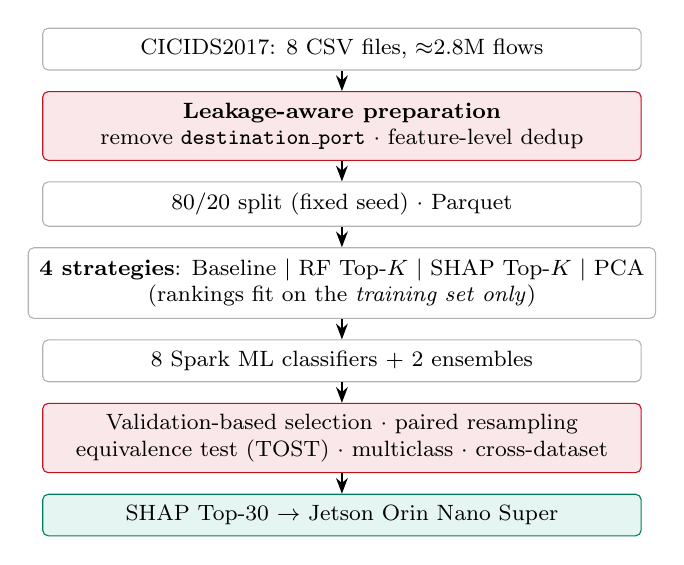
\begin{tikzpicture}[
        font=\footnotesize, node distance=2.6mm, >=Stealth,
        box/.style={draw=gray!60, rounded corners=2pt, align=center, inner sep=4pt, minimum width=7.6cm},
        hl/.style={box, draw=accRed, fill=accRed!10},
        ed/.style={box, draw=accGreen!80!black, fill=accGreen!10},
        arr/.style={-{Stealth[length=2mm]}, semithick}]
        \node[box] (raw)  {CICIDS2017: 8 CSV files, $\approx$2.8M flows};
        \node[hl, below=of raw] (prep) {\textbf{Leakage-aware preparation}\\
              remove \texttt{destination\_port} $\cdot$ feature-level dedup};
        \node[box, below=of prep] (split) {80/20 split (fixed seed) $\cdot$ Parquet};
        \node[box, below=of split] (strat) {\textbf{4 strategies}: Baseline $|$ RF Top-$K$ $|$ SHAP Top-$K$ $|$ PCA\\
              (rankings fit on the \emph{training set only})};
        \node[box, below=of strat] (clf) {8 Spark ML classifiers $+$ 2 ensembles};
        \node[hl, below=of clf] (val) {Validation-based selection $\cdot$ paired resampling\\
              equivalence test (TOST) $\cdot$ multiclass $\cdot$ cross-dataset};
        \node[ed, below=of val] (edge) {SHAP Top-30 $\rightarrow$ Jetson Orin Nano Super};
        \draw[arr] (raw)--(prep); \draw[arr] (prep)--(split); \draw[arr] (split)--(strat);
        \draw[arr] (strat)--(clf); \draw[arr] (clf)--(val); \draw[arr] (val)--(edge);
      \end{tikzpicture}}
    \end{column}
    \begin{column}{0.47\textwidth}
      \textbf{Removals happen \emph{before} the split}
      \begin{itemize}\small
        \item Feature-identical groups with \bad{conflicting labels} are
              dropped \emph{entirely}: \num{270 groups, 44{,}260 rows}.
        \item Result: 77 features, 1.79M / 0.45M train/test flows.
      \end{itemize}
      \vspace{0.2em}
      \textbf{Design fixed \emph{a priori}}
      \begin{itemize}\small
        \item Exploration ($K$ sweep) separated from confirmation.
        \item Hyper-parameters shared across all methods.
        \item The test set enters \bad{no} selection step.
      \end{itemize}
    \end{column}
  \end{columns}
  \note{Deterministic deduplication is the part people get wrong. Conflicting
  groups are removed wholesale, so the result does not depend on how Spark
  partitions the data.}
\end{frame}

% ---------------------------------------------------------------- 1:00
% =====================================================================
\section{III.\ RESULTS AND CONCLUSION}
% =====================================================================

\begin{frame}{Result 1: 60\% of the features are removable}
  \begin{columns}[T]
    \begin{column}{0.55\textwidth}
      \centering\small
      \fitwidth{%
      \begin{tabular}{llccc}
        \toprule
        Method & Model & F1 & Train (s) & Feat. \\
        \midrule
        Baseline           & XGBoost & 0.9971 & 4615.5 & 77 \\
        \textbf{SHAP Top-30} & XGBoost & \num{0.9970} & \num{1226.1} & \num{30} \\
        PCA $k{=}40$         & XGBoost & 0.9939 & 1444.8 & 40 \\
        RF Top-30          & XGBoost & 0.9922 & 1295.1 & 30 \\
        \bottomrule
      \end{tabular}
      }
      \par{\scriptsize One run on the original train/test split. Train (s):
      Spark cluster of 2$\times$ Jetson Orin Nano Super, host as master only.}
      \vspace{0.5em}

      \footnotesize
      \fitwidth{%
      \begin{tabular}{lccc}
        \toprule
        F1 by algorithm & RF Top-30 & SHAP Top-30 & $\Delta$F1 \\
        \midrule
        Random Forest & 0.9879 & 0.9955 & \good{$+$0.008} \\
        XGBoost       & 0.9922 & 0.9970 & \good{$+$0.005} \\
        GBT           & 0.9844 & 0.9918 & \good{$+$0.007} \\
        Decision Tree & 0.9835 & 0.9948 & \good{$+$0.011} \\
        \bottomrule
      \end{tabular}
      }
    \end{column}
    \begin{column}{0.43\textwidth}
      \begin{itemize}\small
        \item SHAP Top-30 keeps baseline F1 while cutting \good{$\approx$60\%
              of features} and \good{$\approx$73\% of training time}.
        \item At \emph{equal} feature count, SHAP beats RF Importance on every
              tree-based algorithm.
        \item PCA uses $k{=}40$ because it \emph{extracts} rather than
              \emph{selects}: each component carries only part of the
              variance. Cheaper than the baseline, but not explainable.
      \end{itemize}
    \end{column}
  \end{columns}
  \note{Two tables, one message: SHAP Top-30 is the operating point. Same
  accuracy, 60 percent fewer features, and it is explainable, which matters
  for the SOC analyst and for the edge board downstream.}
\end{frame}

% ---------------------------------------------------------------- 0:40
\begin{frame}{Result 2: equivalence is tested, not asserted}
  \begin{columns}[T]
    \begin{column}{0.47\textwidth}
      \centering\small
      \fitwidth{%
      \begin{tabular}{lc}
        \toprule
        XGBoost & F1, mean of 6 splits \\
        \midrule
        Baseline (77 features) & 0.99734 \\
        SHAP Top-30            & 0.99720 \\
        \midrule
        \textbf{Gap}           & \textbf{$\approx$0.0001} \\
        \bottomrule
      \end{tabular}
      }
      \vspace{0.4em}

      \footnotesize
      \fitwidth{%
      \begin{tabular}{lc}
        \toprule
        Keeping the port & F1 inflation \\
        \midrule
        4 tree models    & $+$0.0007 to $+$0.0017 \\
        2 linear models  & \bad{$+$0.0395 to $+$0.0415} \\
        \bottomrule
      \end{tabular}
      }
    \end{column}
    \begin{column}{0.50\textwidth}
      \begin{itemize}\small
        \item $N{=}6$ paired \emph{resamplings}: both methods see the same
              split each round.
        \item A significance test cannot show two methods are the same, so we
              test \key{equivalence} directly (TOST).
        \item Result: the true gap is \good{below 0.00023 F1} at
              $\alpha = 0.05$.
        \item The port leak was measured on \key{all eight} classifiers, not
              one.
      \end{itemize}
    \end{column}
  \end{columns}
  \takeaway{Baseline and SHAP Top-30 are \key{equivalent}, so explainability and
  cost decide. How much the port inflates F1 depends on the model class.}
  \note{Say the gap first: one ten-thousandth of F1 over six paired splits.
  Then the point: we do not argue from a non-significant p-value, we test
  equivalence. If asked: exact paired permutation over all $2^6$ sign flips
  gives $p = 0.031$, the floor of that test, Cohen's $d \approx 1.94$. TOST
  against a $\pm0.001$ margin fixed in advance, on the Nadeau--Bengio error,
  gives $p = 3.9\times10^{-6}$, and the tightest supported margin is
  $\pm2.3\times10^{-4}$. Port table: per-model rows are in the paper. MLP is
  $+0.0052$ and Naive Bayes $+0.0108$. All later results have the port removed.}
\end{frame}

% ---------------------------------------------------------------- 0:55
\begin{frame}{Result 3: binary F1 hides the rare classes}
  \begin{columns}[c]
    \begin{column}{0.40\textwidth}
      \centering
      \IfFileExists{../../results/ml_09_multiclass_eval/confusion_matrix.png}
        {\includegraphics[width=0.98\textwidth]{confusion_matrix.png}}
        {\fbox{\parbox{0.8\textwidth}{\centering\vspace{1.2cm}
          \texttt{confusion\_matrix.png}\vspace{1.2cm}}}}
    \end{column}
    \begin{column}{0.58\textwidth}
      \centering\footnotesize
      \fitwidth{%
      \begin{tabular}{lccc}
        \toprule
        Class & Support & Recall & F1 \\
        \multicolumn{4}{l}{\scriptsize Random Forest, all 77 features} \\
        \midrule
        Benign                & 380{,}119 & 0.9997 & 0.9989 \\
        DoS Hulk              & 34{,}446  & 0.9904 & 0.9947 \\
        Web -- Brute Force    & 311       & 0.7299 & 0.7323 \\
        Bot                   & 290       & \bad{0.4552} & 0.6256 \\
        Web -- XSS            & 111       & \bad{0.0270} & 0.0526 \\
        Web -- SQL Injection  & 6         & \bad{0.0000} & 0.0000 \\
        \midrule
        \multicolumn{2}{l}{weighted-F1 $=$ 0.998} &
        \multicolumn{2}{l}{\bad{macro-F1 $=$ 0.806}} \\
        \bottomrule
      \end{tabular}
      }
      \par
      \raggedright\footnotesize
      \begin{itemize}\footnotesize
        \setlength{\itemsep}{0pt}
        \item \textbf{Mislabeled but caught}: \good{76\% of XSS} is still
              flagged as an attack.
        \item \textbf{Missed}: all 6 SQL Injection and \bad{54\% of Bot} are
              predicted benign.
      \end{itemize}
    \end{column}
  \end{columns}
  \note{Random Forest on all 77 features. Weighted F1 0.998 versus macro F1
  0.806. XSS: 81 of 111 land on Web Brute Force, so they are still flagged at
  the binary level. 27 percent of Brute Force also goes to Benign. Three plausible causes. The imbalance is extreme. With the port removed there is no port-80 shortcut, so short HTTP attack flows look like browsing. And Bot C\&C beaconing resembles background traffic. Comparing the reduction
  methods in multiclass mode is future work.}
\end{frame}

% ---------------------------------------------------------------- 0:55
\begin{frame}{Result 4: the scores do not survive a different testbed}
  \begin{columns}[T]
    \begin{column}{0.46\textwidth}
      \centering\small
      \fitwidth{%
      \begin{tabular}{lcc}
        \toprule
        Train $\to$ Test & F1 & AUC-PR \\
        \midrule
        2017 $\to$ 2017 & \good{0.9953} & \good{0.9997} \\
        2017 $\to$ 2018 & \bad{0.03--0.30} & \bad{0.4849} \\
        2018 $\to$ 2018 & \good{0.9246} & \good{0.9679} \\
        2018 $\to$ 2017 & \bad{0.0544} & \bad{0.1926} \\
        \bottomrule
      \end{tabular}
      }
      \\[0.3em]
      \scriptsize
      18 runs of identical code and data. AUC-PR is their mean.
    \end{column}
    \begin{column}{0.50\textwidth}
      \begin{itemize}\small
        \item Cross-dataset AUC-PR drops \bad{1.00$\to$0.48} and
              \bad{0.97$\to$0.19}.
        \item Recall 0.07 / 0.03: the model \key{misses} the other testbed's
              attacks.
        \item Same code, same data, \key{two F1 bands}: 11 runs at
              0.03--0.08, 7 at 0.19--0.30, none between.
        \item Label-free adaptation (scaler refit, CORAL): \bad{F1 0}.
              Retraining on \key{1\% target labels}: \good{0.92 / 0.99}.
      \end{itemize}
    \end{column}
  \end{columns}
  \takeaway{Near-perfect in-domain scores, \emph{even leakage-free ones}, do not certify deployability under distribution shift.}
  \note{Do not soften this. In-domain 0.99, cross-dataset AUC-PR 0.48 / 0.19.
  Recall 0.073 / 0.030 at precision 0.772 / 0.272: it misses attacks rather
  than alarming indiscriminately.
  If asked about the two F1 bands: AUC-PR is the same in both, so the ranking
  does not change between runs, only where the 0.5 threshold falls against a
  cluster of near-identical flows. A mean (0.13) would sit in the empty gap, so
  we report both bands and judge the collapse on AUC-PR. Causes of the shift:
  CICFlowMeter version, network configuration, attack tooling. 1\% of the
  target is about 19k flows. Consistent with prior cross-dataset IDS studies,
  and the reason domain adaptation is a prerequisite rather than a
  nice-to-have.}
\end{frame}

% ---------------------------------------------------------------- 0:40
\begin{frame}{Conclusion}
  \begin{columns}[T]
    \begin{column}{0.52\textwidth}
      \textbf{What we showed}
      \begin{itemize}
        \item SHAP Top-30 retains baseline F1 with \good{$\approx$60\% fewer
              features}.
        \item Baseline vs.\ SHAP Top-30 are \key{equivalent} within
              $\pm2.3\times10^{-4}$ F1.
        \item \bad{macro-F1 0.806} against weighted-F1 0.998.
        \item Cross-dataset AUC-PR \bad{collapses to 0.48 / 0.19}. Retraining on 1\% of target labels recovers it.
      \end{itemize}
    \end{column}
    \begin{column}{0.45\textwidth}
      \textbf{The contribution}
      \begin{itemize}\small
        \item \key{How to evaluate reliably}, as much as which method wins.
      \end{itemize}
      \textbf{Next}
      \begin{itemize}\small
        \item Full CSE-CIC-IDS2018 and newer sets (RoEduNet, CIC-IoT).
        \item Does the SHAP Top-30 \emph{set itself} transfer?
        \item An ablation of the deduplication step.
      \end{itemize}
    \end{column}
  \end{columns}
  \vfill
  \centering \key{Thank you. Questions?}
  \note{Close on the protocol, not the leaderboard.}
\end{frame}

% ---------------------------------------------------------------- 7:00
\begin{frame}{Key references}
  \begin{itemize}\scriptsize
    \setlength{\itemsep}{0.1em}
    \item[{[1]}] Sharafaldin, I., Lashkari, A.\,H. \& Ghorbani, A.\,A.
          \emph{Toward generating a new intrusion detection dataset and
          intrusion traffic characterization}. ICISSP 2018.
          \hfill{\key{CICIDS2017}}
    \item[{[2]}] Lanvin, M. et al. \emph{Errors in the CICIDS2017 Dataset and the
          Significant Differences in Detection Performances It Makes}.
          CRiSIS 2022.
          \hfill{\key{label conflicts}}
    \item[{[3]}] Arp, D. et al. \emph{Dos and Don'ts of Machine Learning in Computer
          Security}. USENIX Security 2022.
          \hfill{\key{leakage pitfalls}}
    \item[{[4]}] Lundberg, S.\,M. \& Lee, S.-I. \emph{A unified approach to
          interpreting model predictions}. NeurIPS 2017.
          \hfill{\key{SHAP}}
    \item[{[5]}] Nadeau, C. \& Bengio, Y. \emph{Inference for the Generalization
          Error}. Machine Learning 52(3), 2003.
          \hfill{\key{corrected CI}}
    \item[{[6]}] D'hooge, L. et al. \emph{Inter-dataset generalization strength of
          supervised machine learning methods for intrusion detection}.
          J.\ Information Security and Applications 54, 2020.
          \hfill{\key{cross-dataset}}
    \item[{[7]}] Zaharia, M. et al. \emph{Spark: Cluster computing with working
          sets}. HotCloud 2010.
          \hfill{\key{Spark ML}}
    \item[{[8]}] CIC \& CSE. \emph{CSE-CIC-IDS2018 dataset}. 2018.
          \hfill{\key{cross-dataset target}}
    \item[{[9]}] Schuirmann, D.\,J. \emph{A comparison of the two one-sided tests
          procedure and the power approach for assessing the equivalence of
          average bioavailability}. J.\ Pharmacokinetics and
          Biopharmaceutics 15(6), 1987.
          \hfill{\key{TOST}}
    \item[{[10]}] Sun, B., Feng, J. \& Saenko, K. \emph{Return of frustratingly
          easy domain adaptation}. AAAI 2016.
          \hfill{\key{CORAL}}
  \end{itemize}
  \note{Not presented. Shown while taking questions, so sources are on
  screen if the audience asks. Full list is in the paper.}
\end{frame}

% =====================================================================
\appendix

\begin{frame}[standout]
  Backup slides
\end{frame}

\begin{frame}{Backup: F1 heatmap, method $\times$ algorithm}
  \centering
  \IfFileExists{../../results/ml_07_cross_method_comparison/f1_heatmap.png}
    {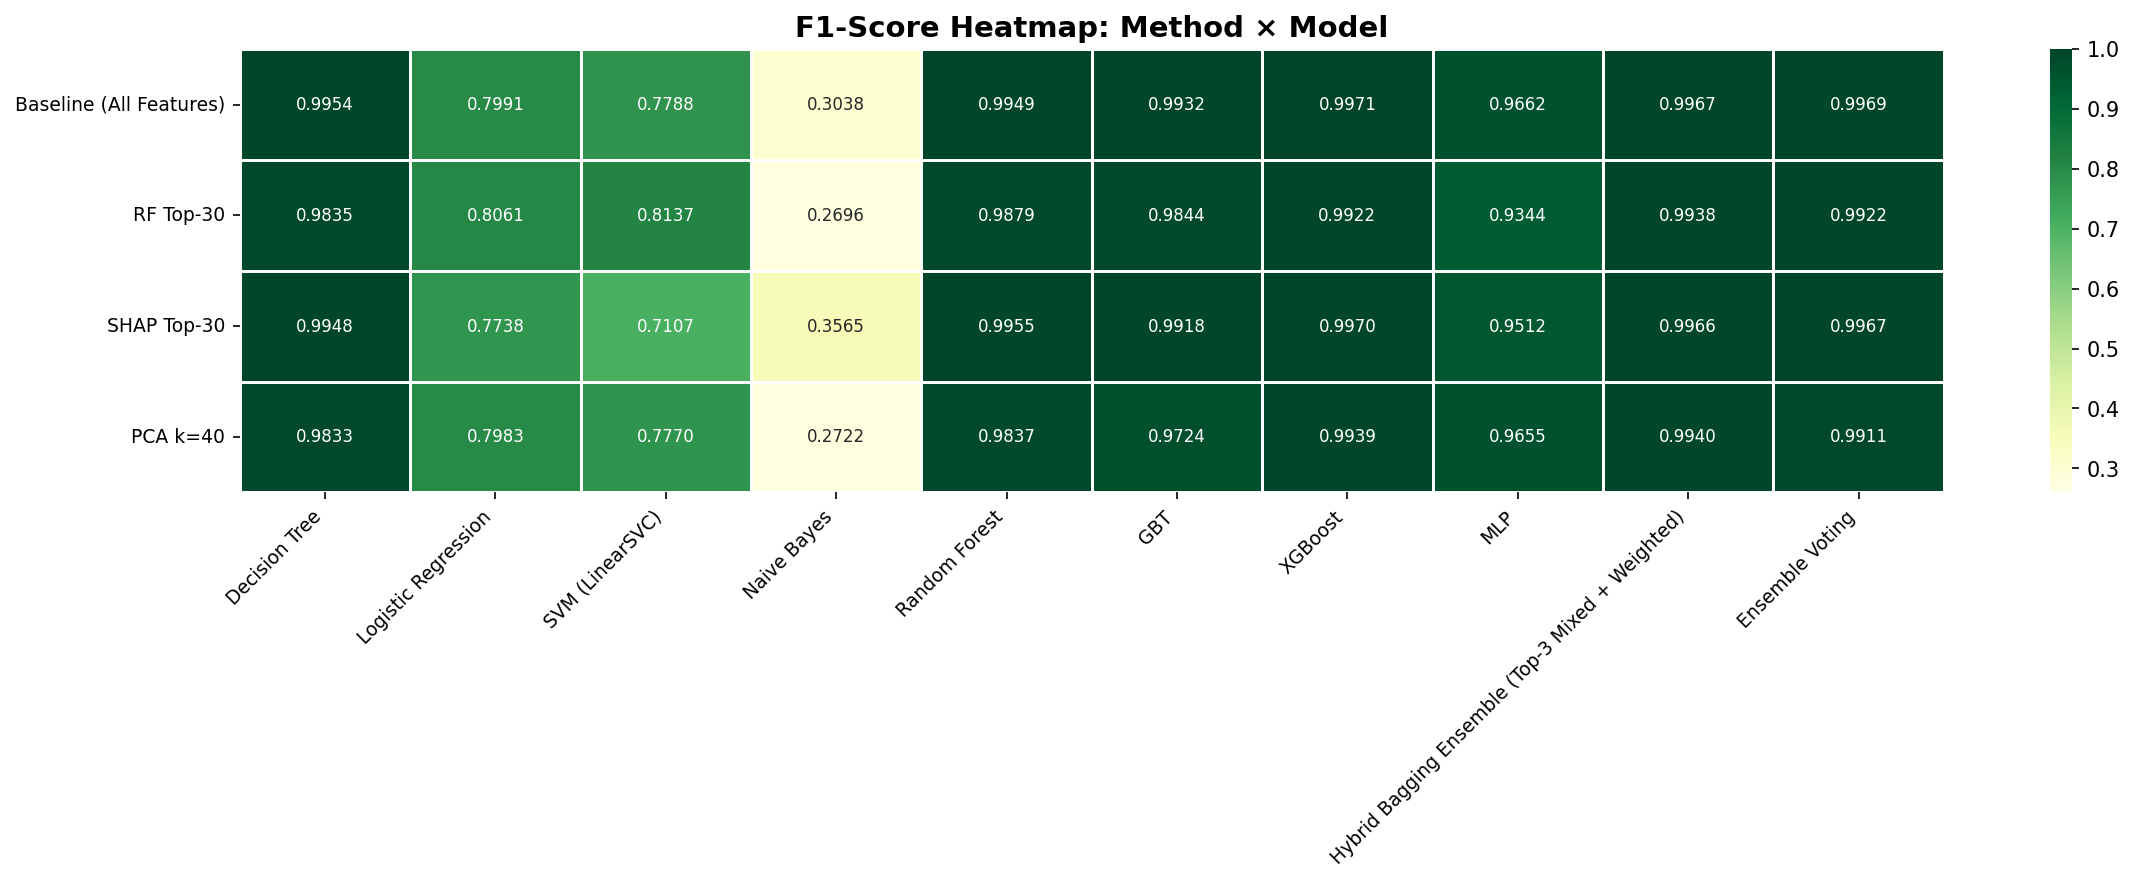
\includegraphics[height=0.74\textheight, width=\textwidth, keepaspectratio]{f1_heatmap.png}}
    {\fbox{\parbox{0.7\textwidth}{\centering\vspace{1.5cm}
      \texttt{f1\_heatmap.png}\vspace{1.5cm}}}}
  \\[0.2em]\footnotesize Binary, port removed. 8 algorithms $\times$ 4 methods.
\end{frame}

\begin{frame}{Backup: hyper-parameters, fixed a priori}
  \centering\footnotesize
  \fitwidth{%
  \begin{tabular}{ll}
    \toprule
    Model & Main hyper-parameters \\
    \midrule
    Decision Tree       & maxDepth=15, minInstancesPerNode=5, impurity=entropy \\
    Logistic Regression & maxIter=200, regParam=0.001, L2, threshold=0.5 \\
    SVM (LinearSVC)     & maxIter=200, regParam=0.001 \\
    Naive Bayes         & gaussian, smoothing=1.0 \\
    Random Forest       & numTrees=200, maxDepth=15, featureSubset=sqrt \\
    GBT                 & maxIter=150, maxDepth=6, stepSize=0.05, subsample=0.8 \\
    XGBoost             & n\_estimators=300, max\_depth=8, lr=0.05, subsample=0.8, colsample=0.8 \\
    MLP                 & layers=[$d$,64,32,2], maxIter=150, stepSize=0.01 \\
    \bottomrule
  \end{tabular}
  }
  \\[0.4em]
  \raggedright\footnotesize
  Shared across all reduction methods, so differences reflect the
  \emph{method}, not per-model tuning. Class weights for 6 models,
  \texttt{scale\_pos\_weight} for XGBoost. MLP is unweighted (Spark ML has no sample weights for it), as stated in the limitations. LightGBM excluded: its
  SynapseML native library is x86\_64-only, and the deployment target is ARM64.
\end{frame}

\begin{frame}{Backup: training and prediction cost}
  \centering
  \IfFileExists{../../results/ml_07_cross_method_comparison/train_predict_time.png}
    {\includegraphics[height=0.68\textheight, width=\textwidth, keepaspectratio]{train_predict_time.png}}
    {\fbox{\parbox{0.7\textwidth}{\centering\vspace{1.5cm}
      \texttt{train\_predict\_time.png}\vspace{1.5cm}}}}
  \\[0.2em]\footnotesize
  Measured on the Spark training cluster. Latency/throughput \emph{on the edge
  device} belong to the companion systems paper.
\end{frame}

\begin{frame}{Backup: threats to validity}
  \begin{itemize}\small
    \item \textbf{Internal.} RF/SHAP rankings come from the original training
          set and stay fixed across resamplings, consistent with the
          a-priori design, but a possible leak in the ranking step. Re-ranking
          inside two of the six resamplings moved F1 by $\le 7.4\times10^{-5}$,
          and 25--26 of 30 features were reselected. MLP carries the
          unweighted-training caveat.
    \item \textbf{External.} CICIDS2017 may not reflect current traffic, and
          benchmark NIDS datasets have documented quality limitations. The
          cross-dataset conclusion rests on a \emph{stratified sample} of
          CSE-CIC-IDS2018. Evasive traffic untested. Feature-level dedup itself
          shifts the benign/attack distribution.
    \item \textbf{Statistical.} $N{=}6$ gives low power: two-sided exact
          enumeration floors $p$ at $2/2^N$, so $N{=}6$ \emph{just} reaches
          0.05. The equivalence claim does not rest on that $p$ but on TOST,
          on the Nadeau--Bengio error that accounts for overlapping
          resamplings. Cross-dataset F1 is not deterministic across runs, so
          it is reported over 18 runs.
  \end{itemize}
\end{frame}

\begin{frame}{Backup: SHAP feature attribution}
  \centering
  \IfFileExists{../../results/ml_06_feature_selection_shap/shap_summary_beeswarm.png}
    {\includegraphics[height=0.68\textheight, width=\textwidth, keepaspectratio]{shap_summary_beeswarm.png}}
    {\fbox{\parbox{0.7\textwidth}{\centering\vspace{1.5cm}
      \texttt{shap\_summary\_beeswarm.png}\vspace{1.5cm}}}}
  \\[0.2em]\footnotesize
  SHAP is computed on a \emph{class-stratified} sample so both benign and
  attack traffic are represented in the ranking.
\end{frame}

\end{document}
"
% ---------------------------------------------------------------------
\ifdefined\shownotes
  \usepackage{pgfpages}
  \setbeameroption{show notes on second screen=right}
\fi

\centeredtitles

\graphicspath{%
  {../../results/ml_07_cross_method_comparison/}%
  {../../results/ml_05_shap_explainability/}%
  {../../results/ml_06_feature_selection_shap/}%
  {../../results/ml_09_multiclass_eval/}%
  {../../results/ml_10_leakage_ablation/}%
  {../../results/ml_11_cross_dataset/}%
}

\title{Dimensionality Reduction and Feature Selection for Network Intrusion Detection on Apache Spark ML}
\subtitle{\ldots with a Leakage-Aware Evaluation Pipeline}
\author{\textbf{Thai Nguyen Vu}\inst{1} \and Bui Van Dung\inst{2} \and Tri Nhut Do\inst{2} \and Van Du Nguyen\inst{3}}
\institute{\scriptsize
           \inst{1}Campus in Ho Chi Minh City, University of Transport and Communications, Ho Chi Minh City, Vietnam \\
           \inst{2}University of Information Technology, VNU-HCM, Ho Chi Minh City, Vietnam \\
           \inst{3}Faculty of Information Technology, Nong Lam University, Ho Chi Minh City, Vietnam}
\date{FAIR'2026}

\begin{document}

% ---------------------------------------------------------------- 0:20
\maketitle
\note{Seven minutes on a single claim: on CICIDS2017, a near-perfect F1 is
usually a property of the evaluation pipeline, not of the model.}

% ---------------------------------------------------------------- 0:50
% =====================================================================
\section{I.\ PROBLEM AND CONTRIBUTIONS}
% =====================================================================

\begin{frame}{A near-perfect F1 on CICIDS2017 is a warning sign}
  \begin{columns}[T]
    \begin{column}{0.55\textwidth}
      \textbf{Two problems, usually treated separately}
      \begin{itemize}
        \item \key{Cost.} $\approx$80 features per flow.
        \item \key{Trust.} Near-perfect binary F1 usually signals
              \bad{data leakage}.
      \end{itemize}
      \vspace{0.5em}
      \textbf{Two concrete leakage sources}
      \begin{enumerate}
        \item \texttt{destination\_port} encodes the \emph{attacked service}.
        \item \bad{Feature-level duplicates} survive full-row dedup, so the same sample lands in train \emph{and} test.
      \end{enumerate}
    \end{column}
    \begin{column}{0.42\textwidth}
      \begin{alertblock}{This paper}
        Compare four reduction strategies over the same eight Spark ML
        classifiers, but first make the \emph{evaluation pipeline} trustworthy.
      \end{alertblock}
      \begin{exampleblock}{The contribution is the protocol}
        Not ``which method wins'' but \key{how to measure so the answer means
        something}.
      \end{exampleblock}%
    \end{column}
  \end{columns}
  \note{Frame the talk as a measurement paper. The port gives the model a
  port-to-label shortcut, and 80 features are expensive to train, to score and to
  fit on an edge device. Both leakage sources are removed before any split.}
\end{frame}

% ---------------------------------------------------------------- 0:35
\begin{frame}{Contributions}
  \begin{enumerate}
    \item A \key{uniform comparison} of RF Importance, SHAP and PCA across the
          same 8 Spark ML algorithms $+$ 2 ensembles on CICIDS2017.
    \item SHAP contrasted \key{directly} against RF Importance on the same
          training set.
    \item A \key{leakage-aware, statistically tested} pipeline: leak removal,
          deterministic feature-level dedup, validation-based selection, paired
          resampling with an \emph{equivalence} test (TOST).
    \item A \key{per-attack-type} and a \key{cross-dataset} evaluation, which expose what in-domain binary F1 hides.
    \item An \key{edge-aware} recommendation: F1 \emph{and} feature count
          \emph{and} model size, for a Jetson Orin Nano Super (deployment
          reported in a companion systems paper).
  \end{enumerate}
  \note{Five contributions. Three, four and five are the ones rarely done
  together.}
\end{frame}

% ---------------------------------------------------------------- 0:55
% =====================================================================
\section{II.\ LEAKAGE-AWARE PIPELINE}
% =====================================================================

\begin{frame}{The leakage-aware pipeline}
  \begin{columns}[c]
    \begin{column}{0.5\textwidth}
      \centering
      \resizebox{0.98\textwidth}{!}{%
      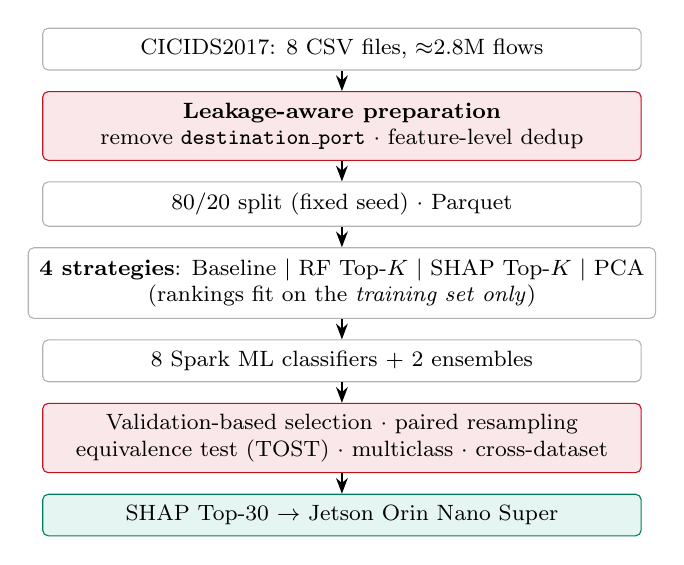
\begin{tikzpicture}[
        font=\footnotesize, node distance=2.6mm, >=Stealth,
        box/.style={draw=gray!60, rounded corners=2pt, align=center, inner sep=4pt, minimum width=7.6cm},
        hl/.style={box, draw=accRed, fill=accRed!10},
        ed/.style={box, draw=accGreen!80!black, fill=accGreen!10},
        arr/.style={-{Stealth[length=2mm]}, semithick}]
        \node[box] (raw)  {CICIDS2017: 8 CSV files, $\approx$2.8M flows};
        \node[hl, below=of raw] (prep) {\textbf{Leakage-aware preparation}\\
              remove \texttt{destination\_port} $\cdot$ feature-level dedup};
        \node[box, below=of prep] (split) {80/20 split (fixed seed) $\cdot$ Parquet};
        \node[box, below=of split] (strat) {\textbf{4 strategies}: Baseline $|$ RF Top-$K$ $|$ SHAP Top-$K$ $|$ PCA\\
              (rankings fit on the \emph{training set only})};
        \node[box, below=of strat] (clf) {8 Spark ML classifiers $+$ 2 ensembles};
        \node[hl, below=of clf] (val) {Validation-based selection $\cdot$ paired resampling\\
              equivalence test (TOST) $\cdot$ multiclass $\cdot$ cross-dataset};
        \node[ed, below=of val] (edge) {SHAP Top-30 $\rightarrow$ Jetson Orin Nano Super};
        \draw[arr] (raw)--(prep); \draw[arr] (prep)--(split); \draw[arr] (split)--(strat);
        \draw[arr] (strat)--(clf); \draw[arr] (clf)--(val); \draw[arr] (val)--(edge);
      \end{tikzpicture}}
    \end{column}
    \begin{column}{0.47\textwidth}
      \textbf{Removals happen \emph{before} the split}
      \begin{itemize}\small
        \item Feature-identical groups with \bad{conflicting labels} are
              dropped \emph{entirely}: \num{270 groups, 44{,}260 rows}.
        \item Result: 77 features, 1.79M / 0.45M train/test flows.
      \end{itemize}
      \vspace{0.2em}
      \textbf{Design fixed \emph{a priori}}
      \begin{itemize}\small
        \item Exploration ($K$ sweep) separated from confirmation.
        \item Hyper-parameters shared across all methods.
        \item The test set enters \bad{no} selection step.
      \end{itemize}
    \end{column}
  \end{columns}
  \note{Deterministic deduplication is the part people get wrong. Conflicting
  groups are removed wholesale, so the result does not depend on how Spark
  partitions the data.}
\end{frame}

% ---------------------------------------------------------------- 1:00
% =====================================================================
\section{III.\ RESULTS AND CONCLUSION}
% =====================================================================

\begin{frame}{Result 1: 60\% of the features are removable}
  \begin{columns}[T]
    \begin{column}{0.55\textwidth}
      \centering\small
      \fitwidth{%
      \begin{tabular}{llccc}
        \toprule
        Method & Model & F1 & Train (s) & Feat. \\
        \midrule
        Baseline           & XGBoost & 0.9971 & 4615.5 & 77 \\
        \textbf{SHAP Top-30} & XGBoost & \num{0.9970} & \num{1226.1} & \num{30} \\
        PCA $k{=}40$         & XGBoost & 0.9939 & 1444.8 & 40 \\
        RF Top-30          & XGBoost & 0.9922 & 1295.1 & 30 \\
        \bottomrule
      \end{tabular}
      }
      \par{\scriptsize One run on the original train/test split. Train (s):
      Spark cluster of 2$\times$ Jetson Orin Nano Super, host as master only.}
      \vspace{0.5em}

      \footnotesize
      \fitwidth{%
      \begin{tabular}{lccc}
        \toprule
        F1 by algorithm & RF Top-30 & SHAP Top-30 & $\Delta$F1 \\
        \midrule
        Random Forest & 0.9879 & 0.9955 & \good{$+$0.008} \\
        XGBoost       & 0.9922 & 0.9970 & \good{$+$0.005} \\
        GBT           & 0.9844 & 0.9918 & \good{$+$0.007} \\
        Decision Tree & 0.9835 & 0.9948 & \good{$+$0.011} \\
        \bottomrule
      \end{tabular}
      }
    \end{column}
    \begin{column}{0.43\textwidth}
      \begin{itemize}\small
        \item SHAP Top-30 keeps baseline F1 while cutting \good{$\approx$60\%
              of features} and \good{$\approx$73\% of training time}.
        \item At \emph{equal} feature count, SHAP beats RF Importance on every
              tree-based algorithm.
        \item PCA uses $k{=}40$ because it \emph{extracts} rather than
              \emph{selects}: each component carries only part of the
              variance. Cheaper than the baseline, but not explainable.
      \end{itemize}
    \end{column}
  \end{columns}
  \note{Two tables, one message: SHAP Top-30 is the operating point. Same
  accuracy, 60 percent fewer features, and it is explainable, which matters
  for the SOC analyst and for the edge board downstream.}
\end{frame}

% ---------------------------------------------------------------- 0:40
\begin{frame}{Result 2: equivalence is tested, not asserted}
  \begin{columns}[T]
    \begin{column}{0.47\textwidth}
      \centering\small
      \fitwidth{%
      \begin{tabular}{lc}
        \toprule
        XGBoost & F1, mean of 6 splits \\
        \midrule
        Baseline (77 features) & 0.99734 \\
        SHAP Top-30            & 0.99720 \\
        \midrule
        \textbf{Gap}           & \textbf{$\approx$0.0001} \\
        \bottomrule
      \end{tabular}
      }
      \vspace{0.4em}

      \footnotesize
      \fitwidth{%
      \begin{tabular}{lc}
        \toprule
        Keeping the port & F1 inflation \\
        \midrule
        4 tree models    & $+$0.0007 to $+$0.0017 \\
        2 linear models  & \bad{$+$0.0395 to $+$0.0415} \\
        \bottomrule
      \end{tabular}
      }
    \end{column}
    \begin{column}{0.50\textwidth}
      \begin{itemize}\small
        \item $N{=}6$ paired \emph{resamplings}: both methods see the same
              split each round.
        \item A significance test cannot show two methods are the same, so we
              test \key{equivalence} directly (TOST).
        \item Result: the true gap is \good{below 0.00023 F1} at
              $\alpha = 0.05$.
        \item The port leak was measured on \key{all eight} classifiers, not
              one.
      \end{itemize}
    \end{column}
  \end{columns}
  \takeaway{Baseline and SHAP Top-30 are \key{equivalent}, so explainability and
  cost decide. How much the port inflates F1 depends on the model class.}
  \note{Say the gap first: one ten-thousandth of F1 over six paired splits.
  Then the point: we do not argue from a non-significant p-value, we test
  equivalence. If asked: exact paired permutation over all $2^6$ sign flips
  gives $p = 0.031$, the floor of that test, Cohen's $d \approx 1.94$. TOST
  against a $\pm0.001$ margin fixed in advance, on the Nadeau--Bengio error,
  gives $p = 3.9\times10^{-6}$, and the tightest supported margin is
  $\pm2.3\times10^{-4}$. Port table: per-model rows are in the paper. MLP is
  $+0.0052$ and Naive Bayes $+0.0108$. All later results have the port removed.}
\end{frame}

% ---------------------------------------------------------------- 0:55
\begin{frame}{Result 3: binary F1 hides the rare classes}
  \begin{columns}[c]
    \begin{column}{0.40\textwidth}
      \centering
      \IfFileExists{../../results/ml_09_multiclass_eval/confusion_matrix.png}
        {\includegraphics[width=0.98\textwidth]{confusion_matrix.png}}
        {\fbox{\parbox{0.8\textwidth}{\centering\vspace{1.2cm}
          \texttt{confusion\_matrix.png}\vspace{1.2cm}}}}
    \end{column}
    \begin{column}{0.58\textwidth}
      \centering\footnotesize
      \fitwidth{%
      \begin{tabular}{lccc}
        \toprule
        Class & Support & Recall & F1 \\
        \multicolumn{4}{l}{\scriptsize Random Forest, all 77 features} \\
        \midrule
        Benign                & 380{,}119 & 0.9997 & 0.9989 \\
        DoS Hulk              & 34{,}446  & 0.9904 & 0.9947 \\
        Web -- Brute Force    & 311       & 0.7299 & 0.7323 \\
        Bot                   & 290       & \bad{0.4552} & 0.6256 \\
        Web -- XSS            & 111       & \bad{0.0270} & 0.0526 \\
        Web -- SQL Injection  & 6         & \bad{0.0000} & 0.0000 \\
        \midrule
        \multicolumn{2}{l}{weighted-F1 $=$ 0.998} &
        \multicolumn{2}{l}{\bad{macro-F1 $=$ 0.806}} \\
        \bottomrule
      \end{tabular}
      }
      \par
      \raggedright\footnotesize
      \begin{itemize}\footnotesize
        \setlength{\itemsep}{0pt}
        \item \textbf{Mislabeled but caught}: \good{76\% of XSS} is still
              flagged as an attack.
        \item \textbf{Missed}: all 6 SQL Injection and \bad{54\% of Bot} are
              predicted benign.
      \end{itemize}
    \end{column}
  \end{columns}
  \note{Random Forest on all 77 features. Weighted F1 0.998 versus macro F1
  0.806. XSS: 81 of 111 land on Web Brute Force, so they are still flagged at
  the binary level. 27 percent of Brute Force also goes to Benign. Three plausible causes. The imbalance is extreme. With the port removed there is no port-80 shortcut, so short HTTP attack flows look like browsing. And Bot C\&C beaconing resembles background traffic. Comparing the reduction
  methods in multiclass mode is future work.}
\end{frame}

% ---------------------------------------------------------------- 0:55
\begin{frame}{Result 4: the scores do not survive a different testbed}
  \begin{columns}[T]
    \begin{column}{0.46\textwidth}
      \centering\small
      \fitwidth{%
      \begin{tabular}{lcc}
        \toprule
        Train $\to$ Test & F1 & AUC-PR \\
        \midrule
        2017 $\to$ 2017 & \good{0.9953} & \good{0.9997} \\
        2017 $\to$ 2018 & \bad{0.03--0.30} & \bad{0.4849} \\
        2018 $\to$ 2018 & \good{0.9246} & \good{0.9679} \\
        2018 $\to$ 2017 & \bad{0.0544} & \bad{0.1926} \\
        \bottomrule
      \end{tabular}
      }
      \\[0.3em]
      \scriptsize
      18 runs of identical code and data. AUC-PR is their mean.
    \end{column}
    \begin{column}{0.50\textwidth}
      \begin{itemize}\small
        \item Cross-dataset AUC-PR drops \bad{1.00$\to$0.48} and
              \bad{0.97$\to$0.19}.
        \item Recall 0.07 / 0.03: the model \key{misses} the other testbed's
              attacks.
        \item Same code, same data, \key{two F1 bands}: 11 runs at
              0.03--0.08, 7 at 0.19--0.30, none between.
        \item Label-free adaptation (scaler refit, CORAL): \bad{F1 0}.
              Retraining on \key{1\% target labels}: \good{0.92 / 0.99}.
      \end{itemize}
    \end{column}
  \end{columns}
  \takeaway{Near-perfect in-domain scores, \emph{even leakage-free ones}, do not certify deployability under distribution shift.}
  \note{Do not soften this. In-domain 0.99, cross-dataset AUC-PR 0.48 / 0.19.
  Recall 0.073 / 0.030 at precision 0.772 / 0.272: it misses attacks rather
  than alarming indiscriminately.
  If asked about the two F1 bands: AUC-PR is the same in both, so the ranking
  does not change between runs, only where the 0.5 threshold falls against a
  cluster of near-identical flows. A mean (0.13) would sit in the empty gap, so
  we report both bands and judge the collapse on AUC-PR. Causes of the shift:
  CICFlowMeter version, network configuration, attack tooling. 1\% of the
  target is about 19k flows. Consistent with prior cross-dataset IDS studies,
  and the reason domain adaptation is a prerequisite rather than a
  nice-to-have.}
\end{frame}

% ---------------------------------------------------------------- 0:40
\begin{frame}{Conclusion}
  \begin{columns}[T]
    \begin{column}{0.52\textwidth}
      \textbf{What we showed}
      \begin{itemize}
        \item SHAP Top-30 retains baseline F1 with \good{$\approx$60\% fewer
              features}.
        \item Baseline vs.\ SHAP Top-30 are \key{equivalent} within
              $\pm2.3\times10^{-4}$ F1.
        \item \bad{macro-F1 0.806} against weighted-F1 0.998.
        \item Cross-dataset AUC-PR \bad{collapses to 0.48 / 0.19}. Retraining on 1\% of target labels recovers it.
      \end{itemize}
    \end{column}
    \begin{column}{0.45\textwidth}
      \textbf{The contribution}
      \begin{itemize}\small
        \item \key{How to evaluate reliably}, as much as which method wins.
      \end{itemize}
      \textbf{Next}
      \begin{itemize}\small
        \item Full CSE-CIC-IDS2018 and newer sets (RoEduNet, CIC-IoT).
        \item Does the SHAP Top-30 \emph{set itself} transfer?
        \item An ablation of the deduplication step.
      \end{itemize}
    \end{column}
  \end{columns}
  \vfill
  \centering \key{Thank you. Questions?}
  \note{Close on the protocol, not the leaderboard.}
\end{frame}

% ---------------------------------------------------------------- 7:00
\begin{frame}{Key references}
  \begin{itemize}\scriptsize
    \setlength{\itemsep}{0.1em}
    \item[{[1]}] Sharafaldin, I., Lashkari, A.\,H. \& Ghorbani, A.\,A.
          \emph{Toward generating a new intrusion detection dataset and
          intrusion traffic characterization}. ICISSP 2018.
          \hfill{\key{CICIDS2017}}
    \item[{[2]}] Lanvin, M. et al. \emph{Errors in the CICIDS2017 Dataset and the
          Significant Differences in Detection Performances It Makes}.
          CRiSIS 2022.
          \hfill{\key{label conflicts}}
    \item[{[3]}] Arp, D. et al. \emph{Dos and Don'ts of Machine Learning in Computer
          Security}. USENIX Security 2022.
          \hfill{\key{leakage pitfalls}}
    \item[{[4]}] Lundberg, S.\,M. \& Lee, S.-I. \emph{A unified approach to
          interpreting model predictions}. NeurIPS 2017.
          \hfill{\key{SHAP}}
    \item[{[5]}] Nadeau, C. \& Bengio, Y. \emph{Inference for the Generalization
          Error}. Machine Learning 52(3), 2003.
          \hfill{\key{corrected CI}}
    \item[{[6]}] D'hooge, L. et al. \emph{Inter-dataset generalization strength of
          supervised machine learning methods for intrusion detection}.
          J.\ Information Security and Applications 54, 2020.
          \hfill{\key{cross-dataset}}
    \item[{[7]}] Zaharia, M. et al. \emph{Spark: Cluster computing with working
          sets}. HotCloud 2010.
          \hfill{\key{Spark ML}}
    \item[{[8]}] CIC \& CSE. \emph{CSE-CIC-IDS2018 dataset}. 2018.
          \hfill{\key{cross-dataset target}}
    \item[{[9]}] Schuirmann, D.\,J. \emph{A comparison of the two one-sided tests
          procedure and the power approach for assessing the equivalence of
          average bioavailability}. J.\ Pharmacokinetics and
          Biopharmaceutics 15(6), 1987.
          \hfill{\key{TOST}}
    \item[{[10]}] Sun, B., Feng, J. \& Saenko, K. \emph{Return of frustratingly
          easy domain adaptation}. AAAI 2016.
          \hfill{\key{CORAL}}
  \end{itemize}
  \note{Not presented. Shown while taking questions, so sources are on
  screen if the audience asks. Full list is in the paper.}
\end{frame}

% =====================================================================
\appendix

\begin{frame}[standout]
  Backup slides
\end{frame}

\begin{frame}{Backup: F1 heatmap, method $\times$ algorithm}
  \centering
  \IfFileExists{../../results/ml_07_cross_method_comparison/f1_heatmap.png}
    {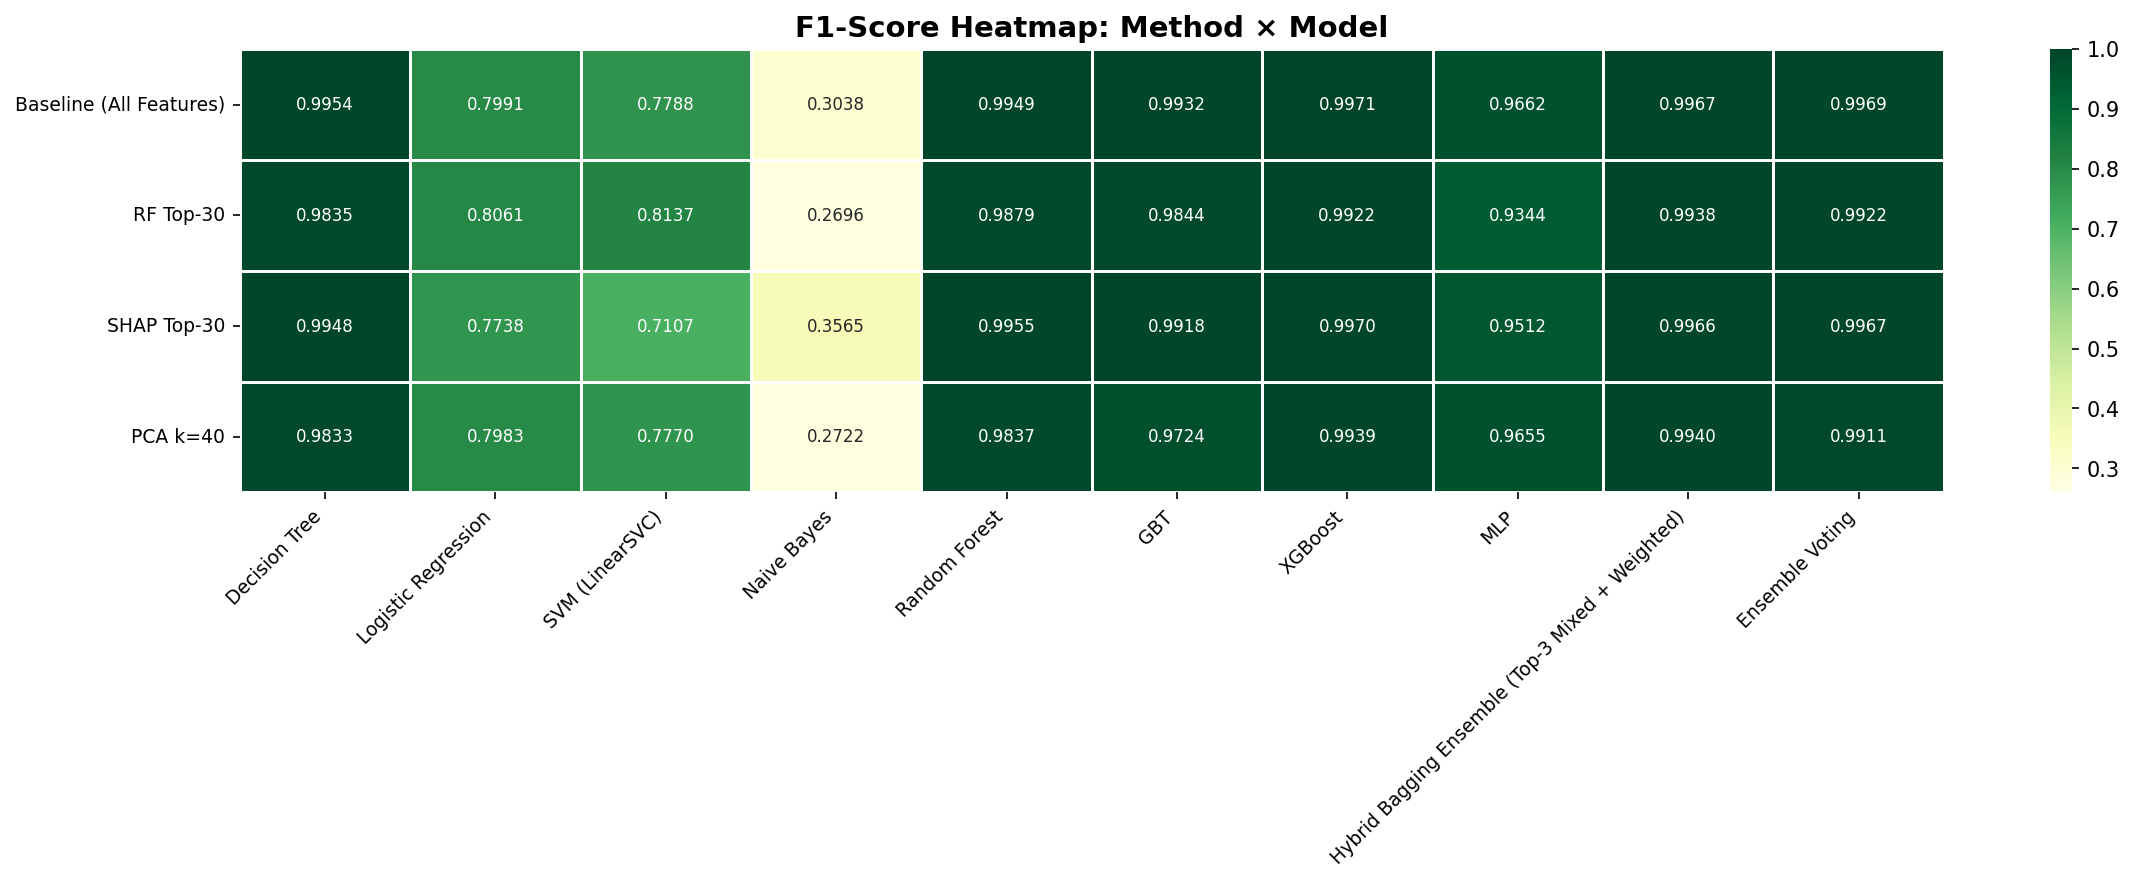
\includegraphics[height=0.74\textheight, width=\textwidth, keepaspectratio]{f1_heatmap.png}}
    {\fbox{\parbox{0.7\textwidth}{\centering\vspace{1.5cm}
      \texttt{f1\_heatmap.png}\vspace{1.5cm}}}}
  \\[0.2em]\footnotesize Binary, port removed. 8 algorithms $\times$ 4 methods.
\end{frame}

\begin{frame}{Backup: hyper-parameters, fixed a priori}
  \centering\footnotesize
  \fitwidth{%
  \begin{tabular}{ll}
    \toprule
    Model & Main hyper-parameters \\
    \midrule
    Decision Tree       & maxDepth=15, minInstancesPerNode=5, impurity=entropy \\
    Logistic Regression & maxIter=200, regParam=0.001, L2, threshold=0.5 \\
    SVM (LinearSVC)     & maxIter=200, regParam=0.001 \\
    Naive Bayes         & gaussian, smoothing=1.0 \\
    Random Forest       & numTrees=200, maxDepth=15, featureSubset=sqrt \\
    GBT                 & maxIter=150, maxDepth=6, stepSize=0.05, subsample=0.8 \\
    XGBoost             & n\_estimators=300, max\_depth=8, lr=0.05, subsample=0.8, colsample=0.8 \\
    MLP                 & layers=[$d$,64,32,2], maxIter=150, stepSize=0.01 \\
    \bottomrule
  \end{tabular}
  }
  \\[0.4em]
  \raggedright\footnotesize
  Shared across all reduction methods, so differences reflect the
  \emph{method}, not per-model tuning. Class weights for 6 models,
  \texttt{scale\_pos\_weight} for XGBoost. MLP is unweighted (Spark ML has no sample weights for it), as stated in the limitations. LightGBM excluded: its
  SynapseML native library is x86\_64-only, and the deployment target is ARM64.
\end{frame}

\begin{frame}{Backup: training and prediction cost}
  \centering
  \IfFileExists{../../results/ml_07_cross_method_comparison/train_predict_time.png}
    {\includegraphics[height=0.68\textheight, width=\textwidth, keepaspectratio]{train_predict_time.png}}
    {\fbox{\parbox{0.7\textwidth}{\centering\vspace{1.5cm}
      \texttt{train\_predict\_time.png}\vspace{1.5cm}}}}
  \\[0.2em]\footnotesize
  Measured on the Spark training cluster. Latency/throughput \emph{on the edge
  device} belong to the companion systems paper.
\end{frame}

\begin{frame}{Backup: threats to validity}
  \begin{itemize}\small
    \item \textbf{Internal.} RF/SHAP rankings come from the original training
          set and stay fixed across resamplings, consistent with the
          a-priori design, but a possible leak in the ranking step. Re-ranking
          inside two of the six resamplings moved F1 by $\le 7.4\times10^{-5}$,
          and 25--26 of 30 features were reselected. MLP carries the
          unweighted-training caveat.
    \item \textbf{External.} CICIDS2017 may not reflect current traffic, and
          benchmark NIDS datasets have documented quality limitations. The
          cross-dataset conclusion rests on a \emph{stratified sample} of
          CSE-CIC-IDS2018. Evasive traffic untested. Feature-level dedup itself
          shifts the benign/attack distribution.
    \item \textbf{Statistical.} $N{=}6$ gives low power: two-sided exact
          enumeration floors $p$ at $2/2^N$, so $N{=}6$ \emph{just} reaches
          0.05. The equivalence claim does not rest on that $p$ but on TOST,
          on the Nadeau--Bengio error that accounts for overlapping
          resamplings. Cross-dataset F1 is not deterministic across runs, so
          it is reported over 18 runs.
  \end{itemize}
\end{frame}

\begin{frame}{Backup: SHAP feature attribution}
  \centering
  \IfFileExists{../../results/ml_06_feature_selection_shap/shap_summary_beeswarm.png}
    {\includegraphics[height=0.68\textheight, width=\textwidth, keepaspectratio]{shap_summary_beeswarm.png}}
    {\fbox{\parbox{0.7\textwidth}{\centering\vspace{1.5cm}
      \texttt{shap\_summary\_beeswarm.png}\vspace{1.5cm}}}}
  \\[0.2em]\footnotesize
  SHAP is computed on a \emph{class-stratified} sample so both benign and
  attack traffic are represented in the ranking.
\end{frame}

\end{document}
